\documentclass{beamer}

\usepackage[T1]{fontenc}
\usepackage[utf8]{inputenc}
\usepackage{listings}
\usepackage{minted}

\title{Tennis genetic algorithm}
\subtitle{Group - Iga Świątek Fanklub}
\author{Magdalena Rąpała \\ Miłosz Liniewiecki}
\institute{AEI faculty}
\date{24.06.2026}

\usetheme{Madrid}
\begin{document}
	
	\frame{\titlepage}
	
	\begin{frame}
		\frametitle{Agenda}
		\tableofcontents
	\end{frame}
	
		
	\section{Introduction to problem and environment}
	\begin{frame}
		\frametitle{Introduction to problem and environment}
		\begin{columns}
			\begin{column}{0.55\textwidth}
				Tennis is an Atari Gymnassium environment with two players.
				\begin{itemize}
					\item Blue player - Game AI, our enemy.
					\item Orange player - Our AI, the one we trained.
				\end{itemize}
				Atari Gymnassium does not give you any data to feed into the genetic algorithm, which is why we used OCAtari for RAM values extraction.
			\end{column}
			\begin{column}{0.45\textwidth}
				\begin{figure}
					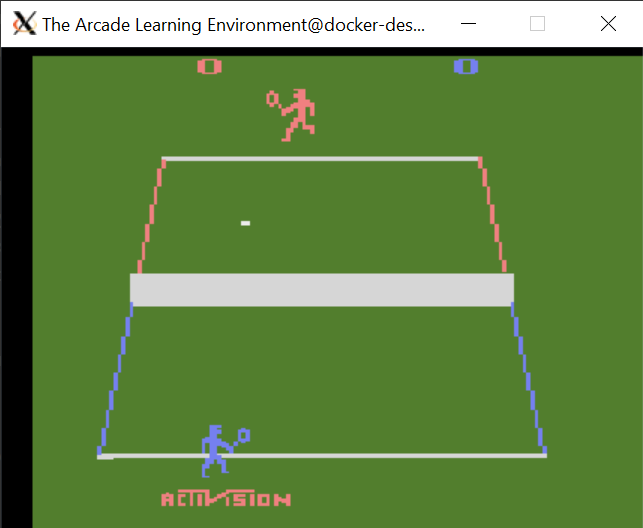
\includegraphics[width=\linewidth]{tennis.png}
					\caption{Tennis environment during training.}
					\label{fig:tennis1}
				\end{figure}
			\end{column}
		\end{columns}
	\end{frame}
	\section{Flowchart}
	{
	\setbeamertemplate{frametitle}{}
	\setbeamertemplate{footline}{}
	\begin{frame}{Flowchart}
		\centering
		\only<1>{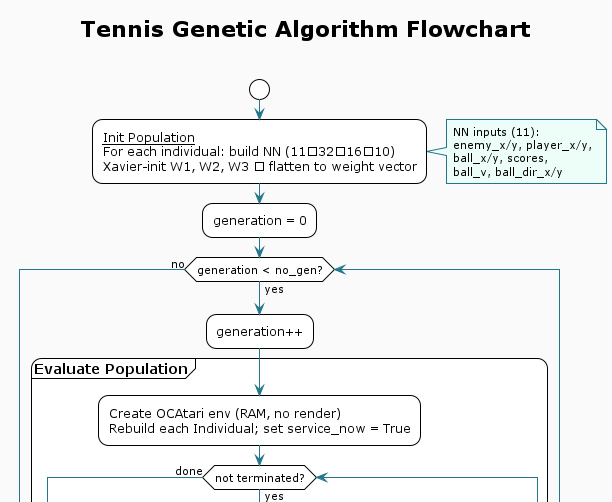
\includegraphics[width=\linewidth,height=\textheight,keepaspectratio]{flowchart1.png}}
		\only<2>{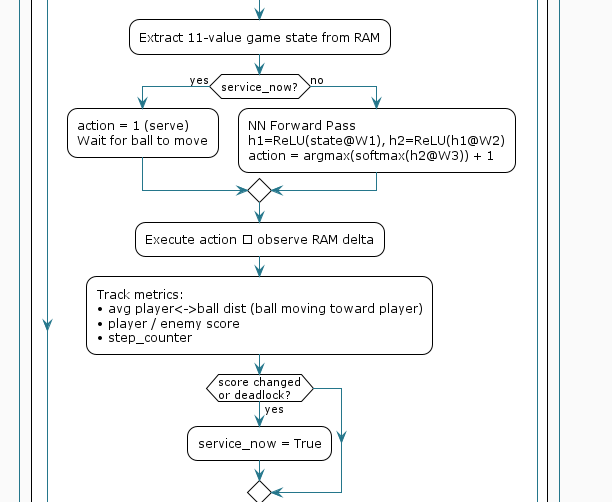
\includegraphics[width=\linewidth,height=\textheight,keepaspectratio]{flowchart2.png}}
		\only<3>{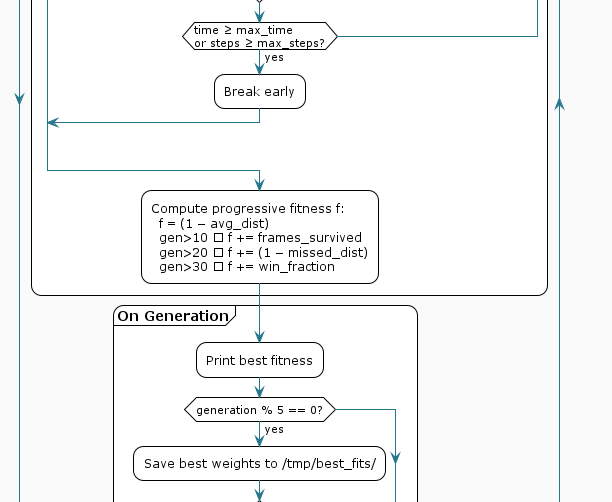
\includegraphics[width=\linewidth,height=\textheight,keepaspectratio]{flowchart3.png}}
		\only<4>{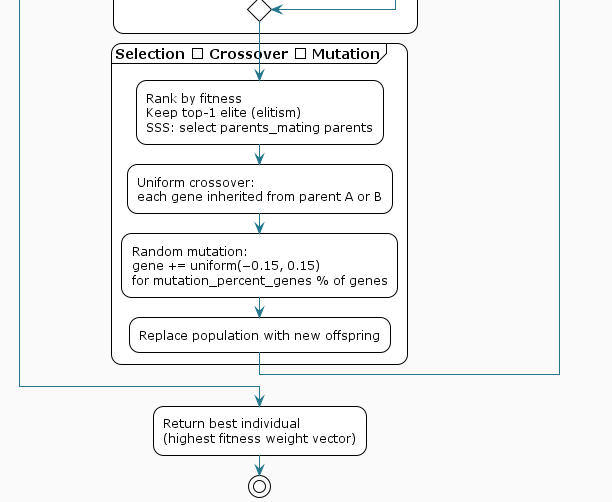
\includegraphics[width=\linewidth,height=\textheight,keepaspectratio]{flowchart4.png}}
	\end{frame}
	}
	\section{Pseudocode}
	\begin{frame}[fragile]
		\frametitle{Pseudocode 1/6 - Init}
		\begin{minted}[fontsize=\footnotesize,linenos]{python}
FUNCTION init_population(no_inv):
population <- []

FOR i = 1 TO no_inv DO
	Build NN with layers: n_x=11 -> h1=32 -> h2=16 -> n_y=10
	Xavier-init weight matrices W1, W2, W3
	population.append(flatten([W1, W2, W3]))
END FOR

RETURN population
		\end{minted}
	\end{frame}
	\begin{frame}[fragile]
		\frametitle{Pseudocode 2/6 - Individual init}
		\begin{minted}[fontsize=\footnotesize,linenos]{python}
population <- init_population(no_inv)
generation <- 0

WHILE generation < no_gen DO

generation <- generation + 1

FOR each individual in population DO

	Create OCAtari "Tennis-v4" env (RAM mode, no render)
	Rebuild Individual from weight vector
	service_now <- True
		\end{minted}
	\end{frame}
	\begin{frame}[fragile]
		\frametitle{Pseudocode 3/6 - State extraction}
		\begin{minted}[fontsize=\footnotesize,linenos,gobble=0]{python}
	WHILE not terminated DO
		state <- extract 11-value game state from RAM
		IF service_now THEN
			action <- 1  (force serve)
			IF ball started moving THEN 
				service_now <- False
			END IF

		ELSE
			h1     <- ReLU(state @ W1)
			h2     <- ReLU(h1    @ W2)
			logits <- h2 @ W3
			action <- argmax(softmax(logits)) + 1
		END IF
		Execute action in env -> observe RAM delta
		\end{minted}
	\end{frame}
	\begin{frame}[fragile]
		\frametitle{Pseudocode 4/6 - Safety checks}
		\begin{minted}[fontsize=\footnotesize,linenos,gobble=0]{python}
		Track metrics:
			avg_player_ball_dist  <- distance(player, ball)
				when ball moves toward player
			player_score, enemy_score
			step_counter <- step_counter + 1

		IF score changed OR deadlock detected THEN
			service_now <- True
		END IF

		IF elapsed_time >= max_time 
			OR step_counter >= max_steps THEN
			BREAK  (early termination)
		END IF

		END WHILE
		\end{minted}
	\end{frame}
	\begin{frame}[fragile]
		\frametitle{Pseudocode 5/6 - Fitness calculation}
		\begin{minted}[fontsize=\footnotesize,linenos,gobble=0]{python}
	Compute fitness f:
	f <- 1 - avg_player_ball_dist
	IF generation > 10 THEN  f <- f + (step_counter / max_steps)
	IF generation > 20 THEN  f <- f + (1 - avg_missed_distance)
	IF generation > 30 THEN  f <- f + (player_score / total_points)

	Store f as fitness of this individual

END FOR
		\end{minted}
	\end{frame}
	\begin{frame}[fragile]
		\frametitle{Pseudocode 6/6 - Selection, best result}
		\begin{minted}[fontsize=\footnotesize,linenos,gobble=0]{python}
Print best fitness of current generation

IF generation MOD 5 = 0 THEN
	Save best weight vector to /tmp/best_fits/gen-{g}-fit-{f}.npy
END IF

Rank population by fitness
elite <- top-1 individual  (preserved unchanged)

parents_mating <- floor(no_inv x parents_frac)
parents <- SSS_select(population, parents_mating)

new_population <- [elite]
		\end{minted}
	\end{frame}
	
	\section{Results}
	\begin{frame}
		\frametitle{Results}
		\begin{figure}
			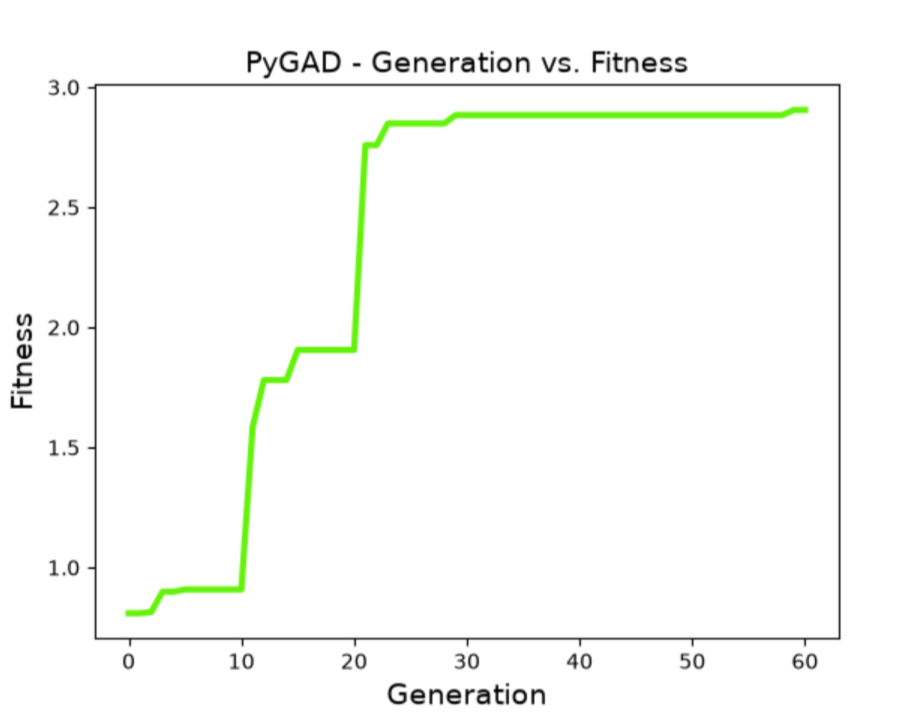
\includegraphics[width=\linewidth,height=0.7\textheight,keepaspectratio]{results.png}
			\caption{Results}
			\label{fig:tennis2}
		\end{figure}
	\end{frame}

\end{document}
